\section{Introduction}
\hspace{2cm} The system is composed of 2 applications, one of them is for the passenger and the other one is for the driver.The user will download the app, then sign up via Email, Name, Password and Phone Number. When the user signs up, his account will be verified via sending a code message to his phone number. And once the user verifies the sent code, he will get his Account. Then, the user has to deposit specific credit in the app's wallet so that the driver can get the receivable payment in case of the user booked a ride then cancelled it
When the user wants to book his ride, he has to select the route line, then the nearest buses to him will be suggested. Then, the system automatically will choose the nearest of all buses and shows this Bus's Passengers. The user will be updated with any change in this number. The system will show all information about the bus and its driver. Also, the user will know the ride cost and how much time the bus driver takes to reach him. The user has the choice to book any number of the bus seats. A feedback of the bus driver will be shown so the user can feel safe and comfortable. When the user confirms the ride, the bus driver will receive a request containing the user's place. Once the bus driver accepts it, the remained time for the bus arrival will be shown for both the user and the driver. The system may send the user a Promo code for free rides or any kind of offers. The user has the right to choose any of his Family or Friends to follow his rides. The system will notify the user and the driver with extra info, instructions or any updates generally. \newline
If a bus driver wants to join Klax, he has to sign up via Email, Name, Password and Phone Number. Then check all needed conditions and tests for applying. Once he gets all conditions and tests successfully done, he gets An Account. If the driver account allows Multiple Route Lines, he has to mention them all and mention the activated one.
And if it allows Private Rides, he has to mention the destinations and the cost. When the driver starts getting passengers for the bus trip, he has to manually add and update the passenger’s number so that the user gets notified. The system automatically add and update the booked rides and seats. When there's is a user's request for a ride, all near drivers get notified. If the driver has enough empty seats, he accepts this request so that the user gets notified.
\newpage
\section{Hardware Components}
\subsection{Server}
\hspace{2cm} Where the process of deploying codes from source control and source artifacts to the platform is done.
\begin{itemize}
    \item Web Server is deployed on Azure Site.
    \item Database is deployed on Atlas Db.
\end{itemize}
\section{Software  Components}
\subsection{Web Server}
\begin{itemize}
    \item The only component that has an access to Persistent Database.
    \item Has the access to External APIs (Paypal and Stripe).
    \item Has the access to Real-Time Database.
    \item Handles the user's requests.
    \item Validates all data before making it allowed in Persistent Database.
\end{itemize}
\subsection{User Software Platform}
\hspace{2cm} The user system is composed of 3 essential sections as following:
\begin{enumerate}
    \item  {\textbf{Home Model}}
    \begin{itemize}
    \item {\textbf{Registration and login}}
    \newline {The user will download the app, then sign up via Email, Name, Password and Phone Number.
When the user signs up, his account will be verified via sending a code message to his phone number.
And once the user verifies the sent code, he will get his Account.}
    \item  {\textbf{User's rides}}
        \newline  {\textbf{past rides}}
        \newline{ Where user can show details of trips and mark any trip as favorite.}
        \begin{itemize}
            \item Mark as favorite option.
            \item Details shown: Trip Line, Date and Time, Trip Duration, Cost, Rating, Car ID.
            \item Sort trips by: Date and Time, Trip line, Rating.
        \end{itemize}
    \item  {\textbf{Free rides}}
    \newline{In Free Rides screen, a user can get a free trips using special codes provided by sponsors and 
partners. The screen includes:}
        \begin{itemize}
           \item Textbox for entering the redemption code.
           \item A send button to send the code to the server along with some user info to be checked if
it’s valid.
           \item A pop-up window as a response to the entered code.
          \item An invitation code for each user that adds a certain cash amount to the user’s wallet if a 
certain user used it, when he signs up.
        \end{itemize}
    
    \item  {\textbf{Settings}}
    \newline{ User can adjust 3 types of settings:}
    \begin{itemize}
        \item {\textbf{Edit Account:}}
        \newline{Where user can show and edit personal details of account.}
        \begin{itemize}
            \item Show or edit name and picture of account user.
            \item Edit password and forgotten password handling.
            \item Show or edit phone and e-mail with verification handling.
        \end{itemize}
        \item {\textbf{Edit App Settings:}}
        \newline{Where user can edit customized settings.}
        \begin{itemize}
            \item Privacy Section
            \newline Notifications pushing: Offers, My Trips, Paired Accounts Trips.
            \item Safety Section
            \newline Verify rides: using PIN.
        \end{itemize}
        \item {\textbf{Family rides}}
        \newline{Where user can show, add, or remove paired family accounts.}
        \begin{figure}[http]%
    \center%
    
\includegraphics[width=0.5\textwidth]{images/ch2/parents.jpg}%
    \caption[Family Rides]{Family Rides}\label{fig: Parents}%
 \end{figure}
        \begin{itemize}
            \item Send Pairing Requests: Search using mobile or email and create a request.
            \item Received Pairing Requests: Accept or refuse.
            \item Remove Paired Accounts.
        \end{itemize}
    \end{itemize}
    \item  {\textbf{Help}}
    \newline{Tutorial on how to use application:}
    \begin{itemize}
        \item Quick Guide to KLAX.
        \item Payment options.
        \item Trips Issues.
    \end{itemize}
\end{itemize}

    \item  {\textbf{Pairing System}}
    \begin{figure}[http]%
    \center%
    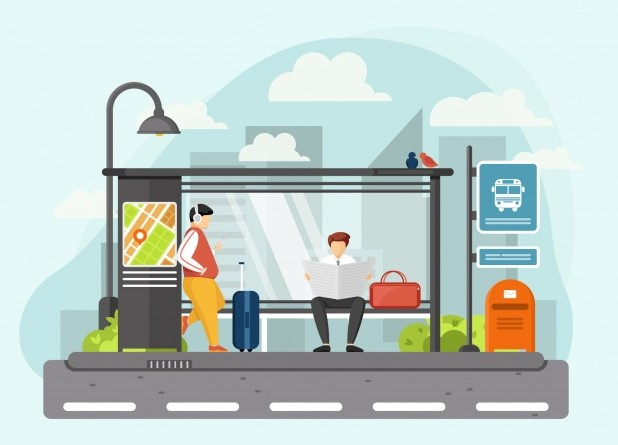
\includegraphics[width=0.5\textwidth]{images/ch2/bus stop.jpg}%
    
    \caption[bus stop]{bus stop}\label{fig: Microbus Station}%
  \end{figure}
  
    \begin{itemize}
        \item  {\textbf{Get request from the user}}
        \newline{When the user wants to book his ride, he has to select the route line, then the nearest buses to him will be suggested.
Then, the system automatically will choose the nearest of all buses and shows this Bus's Passengers.
The user will be updated with any change in this number.
The system will show all information about the bus and its driver. Also, the user will know the ride cost and how much time the bus driver takes to reach him/her.
The user has the choice to book any number of the bus seats.
A feedback of the bus driver will be shown so the user can feel safe and comfortable.
When the user confirms the ride, the bus driver will receive a request containing the user's place.
Once the bus driver accepts it, the remained time for the bus arrival will be shown for both the user and the driver.}

\begin{figure}[http]%
    \center%
    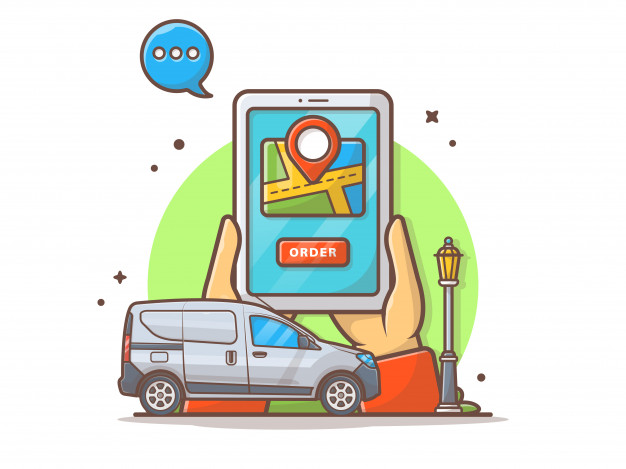
\includegraphics[width=0.5\textwidth]{images/ch2/order.jpg}%
    
    \caption[User's request]{User's request}\label{fig: order}%
 \end{figure}
        \item  {\textbf{Dealing with Database}}
        \newline{The Database filters Klax's drivers by Activation, Reach time and Number of seats. Then the DB chooses the driver, sends request and waits 1m for response.}
        \item  {\textbf{Acceptance scenario}}
        \newline{The user and the driver are tracking each other through the distance between them and the driver contact information. Then they wait for the selected duration and check payment. }
        \newline{The database updates number of seats.}
        \item  {\textbf{Cancellation scenario}}
        \newline{If the driver cancels the user's request, The database will repeat pairing for the same request.}
        \newline{If the user cancels the request after response time, The system will deduct the trip payment from the credit of the user's wallet. }
    \end{itemize}
    \item  {\textbf{Payment System}}
    \newline{A system that allows financial transaction among users and drivers using many different 
payment methods such as: MasterCard, Visa, Vodafone Cash and Fawry.
\begin{figure}[http]%
    \center%
    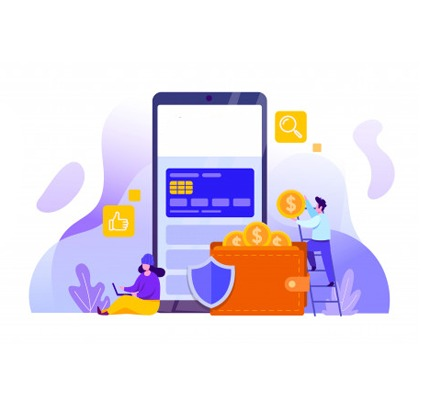
\includegraphics[width=0.5\textwidth]{images/ch2/pay.jpeg}%
    
    \caption[User's Wallet]{User's Wallet}\label{fig: order}%
 \end{figure}
}
\begin{itemize}
    \item {\textbf{User can add credits to his account using one of his personal financial credits:}}
    \newline{ User Login to his financial account. He can add a specific amount of credits by informing current balance and resulting’s balance. Then, money is transferred from his financial account and credits are added to his account.}
    \item{\textbf{Loyal users can borrow money monotonically:}}
    \newline{User sends a request to borrow. The system then checks if this user used the application long enough using his 
number of trips and his rate. 
After making sure money is paid back after several times, user can borrow a larger amount of money}

    \item{\textbf{User can track his status such as:}}
    \begin{itemize}
        \item His current balance
        \item His information about previous 10-20 rides
        \item The last 10 money transfer transactions 
         \item  The sent complains sent and received answers 
    \end{itemize}
    
    \item{\textbf{User can send a request to loan credit from one of his contacts:}}
    \begin{figure}[http]%
    \center%
    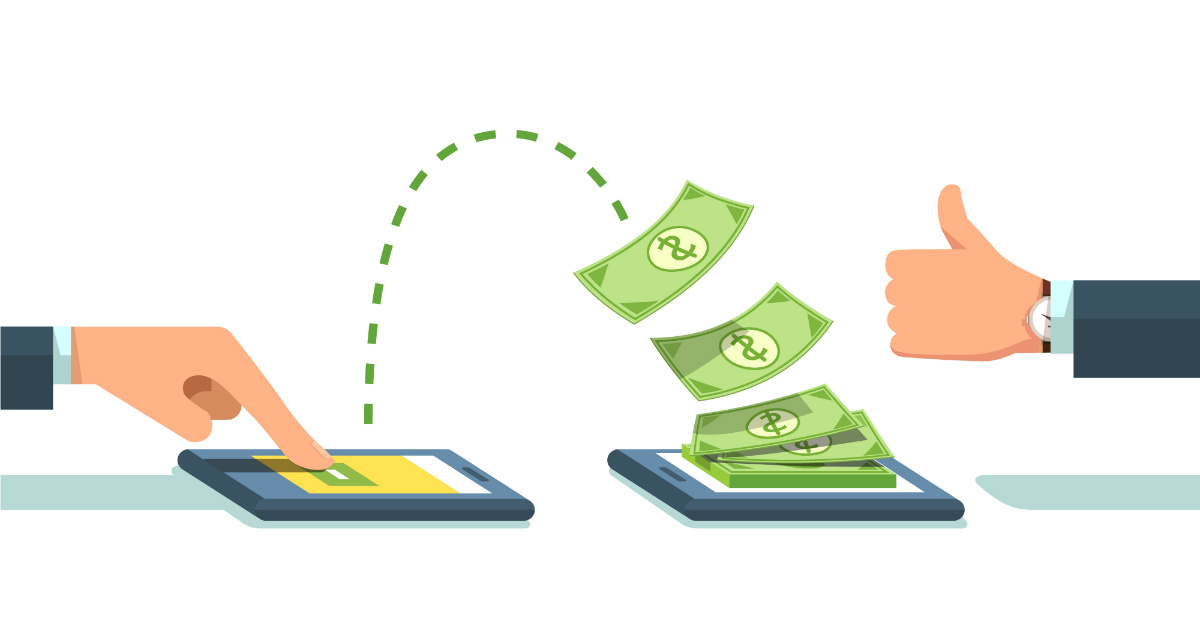
\includegraphics[width=0.5\textwidth]{images/ch2/borrower and loaner.jpg}%
    
    \caption[Loaner and Borrower]{Loaner and borrower}\label{fig: order}%
 \end{figure}
    \newline{Borrower asks for a transfer money request.He fills in the necessary information about the amount to be taken and the chosen 
contact/s. The system process the request and checks if his contact/s have this amount of money. Then, System sends a response with suitability of the chosen contact/s. Borrower is then asked to choose one or more contact to send a request to. Application then sends a request to the loaner. And when loaner sends a response, borrower balance is incremented with the requested amount.}\newline
Loaner receives a notification of a request with details about the borrower and the amount 
of money. He can either accept the request or reject it. If he accepts the borrower's request, Money will be sent. Loaner will be receiving a success notification informing him about the completion of the transaction and his new balance.
    \item{\textbf{ User can send complains about a specific trip 15-20 minutes after the trip was
made:}}
\newline{The user is asked to pick a trip he made. A collecting-information screen appears where user is able to explain his problem. Then his complain is  sent to the system. After handling the complaint, the result is sent to the client as a notification/message to his phone.
\begin{figure}[http]%
    \center%
    
\includegraphics[width=0.5\textwidth]{images/ch2/User's Complain.png}%
    
    \caption[User's Complain]{User's Complain}\label{fig: order}%
 \end{figure}
}
\end{itemize}
    
\end{enumerate}
\subsection{Driver Software Platform}
\hspace{2cm} The driver system is composed of 3 essential sections as following:
\begin{enumerate}
    \item  {\textbf{Home Model}}
    \begin{itemize}
    
       \item {\textbf{Register Form}}
       \newline {If a bus driver wants to join Klax, he has to sign up via Email, Name, Password and Phone Number. Then check all needed conditions and tests for applying. Once he gets all conditions and tests successfully done, he gets An Account.
    If the driver account allows Multiple Route Lines, he has to mention them all and mention the activated one.}
    
       \item {\textbf{Private Trips}}.
       \newline{ a Functionality for the driver to allow passengers to contact him for private trips. This
includes him station-specific lines/places that he is able to travel to.
If it allows Private Rides, he has to mention the destinations and the cost.}

\begin{figure}[http]%
    \center%
    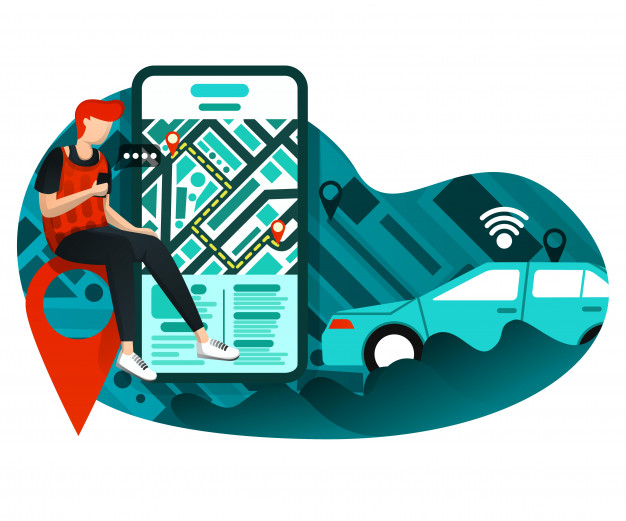
\includegraphics[width=0.5\textwidth]{images/ch2/private.jpg}%
    
    \caption[Private Trips]{Private Trips}\label{fig: Private Trips}%
 \end{figure}
     
    \end{itemize}
    \item  {\textbf{Pairing and Tracking}}
    \begin{itemize}
    
       \item {\textbf{Availability}}
       \newline {The Driver can change its state to whether be available for others see or not.}
       
       \begin{figure}[http]%
    \center%
    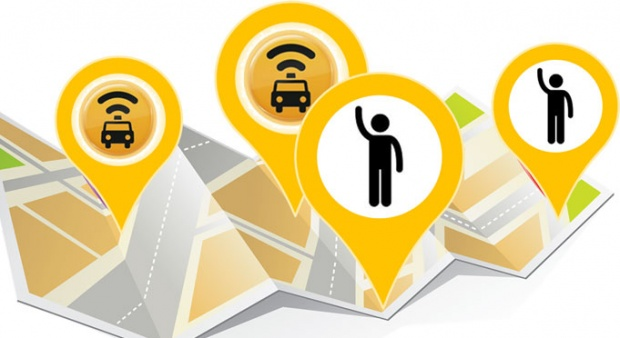
\includegraphics[width=0.5\textwidth]{images/ch2/line.jpg}%
    
    \caption[The driver is online]{The driver is online}\label{fig: The driver is online}%
 \end{figure}
    
       \item {\textbf{Chairs Counter}}.
       \newline{The Driver should be able to change its current used chairs. It does so asking the driver to
add manually offline users from the app, while updating the online users via the app itself and pushing
notification to the driver considering the update.}
       
       \item {\textbf{Trip Ended Mechanism}}.
       \newline{The system to recognize the end of a trip by providing trip feedback from the passenger, a trip is considered done.}
     
    \end{itemize}
    \item  {\textbf{Payments and Complains Model}}
    \begin{itemize}
       \item {\textbf{Earning Statistics}}.
       \newline{ Driver can see his earnings for the past week/month.}
       \item {\textbf{ Feedback System}}
       \newline {Driver should be able to see continuously his feedback.}
       \begin{figure}[http]%
    \center%
    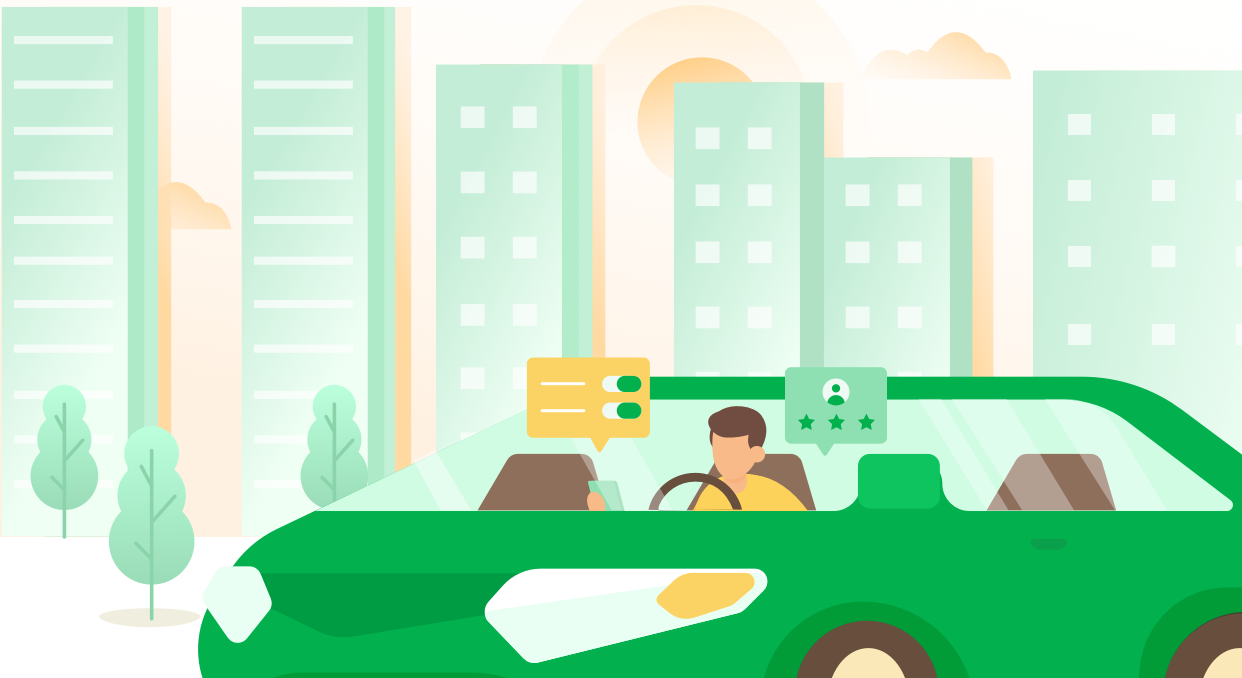
\includegraphics[width=0.5\textwidth]{images/ch2/rate.png}%
    \caption[User's feedback]{User's feedback}\label{fig: User's feedback}%
 \end{figure}
    \end{itemize}
    
\end{enumerate}
\subsection{Admin Software Platform}
\hspace{2cm} It is a website that controls the whole API and the 
notifications sent to users. The site provides the following features:
\begin{itemize}
    \item Statistics: 
    \begin{itemize}
        \item It monitors users, drivers and trips numbers.
        \item Geographic Distribution of passengers according to their governs.
        \item Application Monthly Revenue.
    \end{itemize}
    \item Offers: 
    \newline Makes new offers and promo-codes to users ( discounts, free trips, free cash).
    \item Passenger: 
    \newline Views passengers information.
    \item Tracks driver: 
    \newline Gets every driver live location and make sure he is committed to his route
    \item Complains: 
    \newline Views passengers complaints and send response.
    \item Lines: 
    \newline Adds lines and stations to the application whenever we decide.
\end{itemize}

\subsection{Database}
\hspace{2cm} Database is divided into Persistent Database and Real-time Database.
\begin{itemize}
    \item {\textbf{Persistent Database (Mongo Db)}} 
    \begin{itemize}
        \item Slower.
        \item Used to store the passenger's data, the driver's data and the lines' data.
        \item Accessed only by the server.
        \item Can't be accessed by the user unless he/she sends a request to the server, then the server accepts this request.
    \end{itemize}
    \item {\textbf{Real-time Database (Firebase)}} 
    \begin{itemize}
        \item Used to store the temporary data that need to be updated (The empty seats'number and The driver's location).
        \item Can be accessed by the server, the passenger and the driver.
    \end{itemize}
\end{itemize}
\section{Technologies}
\subsection{Node.JS}
\hspace{2cm} Node.js is a server-side platform built on Google Chrome's JavaScript Engine (V8 Engine). Node.js was developed by Ryan Dahl in 2009 and its latest version is v0.10.36. Node.js is an open source, cross-platform runtime environment for developing server-side and networking applications. Node.js applications are written in JavaScript, and can be run within the Node.js runtime on OS X, Microsoft Windows, and Linux. Node.js also provides a rich library of various JavaScript modules which simplifies the development of web applications using Node.js to a great extent.
\newline{Following are the areas where Node.js is proving itself as a perfect technology partner.}
\begin{itemize}
    \item I/O bound Applications
    \item Data Streaming Applications
    \item Data Intensive Real-time Applications (DIRT)
    \item JSON APIs based Applications
    \item Single Page Applications
\end{itemize}
\textbf{Features of Node.JS}
\begin{enumerate}
    \item {\textbf{Asynchronous and Event Driven}}
    \newline{All APIs of Node.js library ‘re asynchronous, that is, non-blocking. It essentially means a Node.js based server never waits for an API to return data. The server moves to the next API after calling it and a notification mechanism of Events of Node.js helps the server to get a response from the previous API call.}
    \item {\textbf{Very Fast}}
    \newline{Being built on Google Chrome's V8 JavaScript Engine, Node.JS library is very fast in code execution.}
    \item {\textbf{Single Threaded but Highly Scalable}}
    \newline{Node.js uses a single threaded model with event looping. Event mechanism helps the server to respond in a non-blocking way and makes the server highly scalable as opposed to traditional servers which create limited threads to handle requests. Node.js uses a single threaded program and the same program can provide service to a much larger number of requests than traditional servers like Apache HTTP Server}
    \item {\textbf{No Buffering}}
    \newline{Node.JS applications never buffer any data. These applications simply output the data in chunks.}
\end{enumerate}
\textbf{The Node.JS Run-time}
\newline{The source code written in source file is simply JavaScript. The Node.js interpreter will be used to interpret and execute your JavaScript code.
Node.js distribution comes as a binary installable for SunOS, Linux, Mac OS X, and Windows operating systems with the 32-bit (386) and 64-bit (amd64) x86 processor architectures.} \newline \newline
\textbf{Node.JS RESTful API}
\begin{itemize}
    \item {\textbf{REST architecture}}
    \newline{REST is web standard based architecture and uses HTTP Protocol. It revolves around resource where every component is a resource and a resource is accessed by a common interface using HTTP standard methods. REST was first introduced by Roy Fielding in 2000. A REST Server simply provides access to resources and REST client accesses and modifies the resources using HTTP protocol. Here each resource is identified by URIs/ global IDs. REST uses various representation to represent a resource like text, JSON, XML but JSON is the most popular one.}
    \item {\textbf{HTTP Methods}}
    \begin{itemize}
        \item {\textbf{GET}}
        This is used to provide a read only access to a resource.
        \item {\textbf{PUT}}
        This is used to create a new resource.
        \item {\textbf{POST}}
        This is used to update an existing resource or create a new resource.
        \item {\textbf{DELETE}}
        This is used to remove a resource.
    \end{itemize}
    \item {\textbf{RESTful Web Services}}
    \newline{A web service is a collection of open protocols and standards used for exchanging data between applications or systems. Software applications written in various programming languages and running on various platforms can use web services to exchange data over computer networks like the Internet in a manner similar to inter-process communication on a single computer. This interoperability (e.g., communication between Java and Python, or Windows and Linux applications) is due to the use of open standards. \newline
Web services based on REST Architecture are known as RESTful web services. These web services uses HTTP methods to implement the concept of REST architecture. A RESTful web service usually defines a URI, Uniform Resource Identifier a service, which provides resource representation such as JSON and set of HTTP Methods.} \cite{ha001}
\end{itemize}
\subsection{Flutter}
\hspace{2cm} Flutter is an app SDK for building high-performance, high-fidelity apps for iOS, Android, web, and desktop from a single codebase.
The goal is to enable developers to deliver high-performance apps that feel natural on different platforms. We embrace differences in scrolling behaviors, typography, icons, and more.
Apps are written in Dart, which looks familiar if you’ve used a language like Java or JavaScript. Experience with object-oriented languages is definitely helpful.
\newline
\newline{\textbf{Features of Flutter}}
\begin{itemize}
  \item {\textbf{Be highly productive}}
  \begin{itemize}
  \item Develop for IOS and Android from a single codebase
  \item Do more with less code, even on a single OS, with a modern, expressive language and a declarative approach
  \item Prototype and iterate easily
    \begin{itemize}
        \item Experiment by changing code and reloading as your app runs (with hot reload)
        \item Fix crashes and continue debugging from where the app left off
    \end{itemize}
  \end{itemize}
  \item {\textbf{Create beautiful, highly-customized user experiences}}
   \begin{itemize}
  \item oBenefit from a rich set of Material Design and Cupertino (iOS-flavor) widgets built using Flutter’s own framework
  \item oRealize custom, beautiful, brand-driven designs, without the limitations of OEM widget sets
  \end{itemize}
\end{itemize}
\textbf{Core Principles}
\newline{Flutter includes a modern react-style framework, a 2D rendering engine, ready-made widgets, and development tools. These components work together to help you design, build, test, and debug apps. Everything is organized around a few core principles.}
\newline{\textbf{Everything’s a widget}}
\newline{Widgets are the basic building blocks of a Flutter app’s user interface. Each widget is an immutable declaration of part of the user interface. Unlike other frameworks that separate views, view controllers, layouts, and other properties, Flutter has a consistent, unified object model: the widget.
A widget can define:}
\begin{itemize}
  \item a structural element (like a button or menu)
  \item a stylistic element (like a font or color scheme)
  \item an aspect of layout (like padding)
\end{itemize}
Widgets form a hierarchy based on composition. Each widget nests inside, and inherits properties from, its parent. There is no separate “application” object. Instead, the root widget serves this role. You can respond to events, like user interaction, by telling the framework to replace a widget in the hierarchy with another widget. The framework then compares the new and old widgets and efficiently updates the user interface. \cite{ha002}
\subsection{MVC}
\hspace{2cm} The Model View Controller (MVC) is an architectural pattern that separates an application into three main logical components: the model, the view, and the controller. Each of these components are built to handle specific development aspects of an application. MVC is one of the most frequently used industry-standard web development Framework to create scalable and extensible projects.
\begin{figure}[http]%
    \center%
    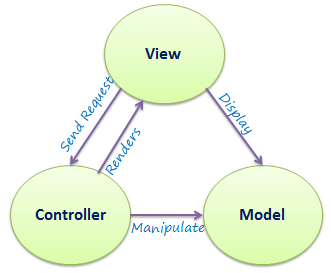
\includegraphics[width=0.5\textwidth]{images/ch2/mvc-architecture.png}%
    \caption[MVC Architecture]{MVC Architecture}\cite{ha003}\label{fig: MVC Architecture}%
  \end{figure}
\newline{\textbf{Model}}
\newline{The Model component corresponds to all the data related logic that the user works with. This can represent either the data that is being transferred between the View and Controller components or any other business logic-related data. For example, a Customer object will retrieve the customer information from the database, manipulate it and update it data back to the database or use it to render data.}
\newline{\textbf{View}}
\newline{The View component is used for all the UI logic of the application. For example, the Customer view will include all the UI components such as text boxes, dropdowns, etc. that the final user interacts with.}
\newline{\textbf{Controller}}
\newline{Controllers act as an interface between Model and View components to process all the business logic and incoming requests, manipulate data using the Model component and interact with the Views to render the final output. For example, the Customer controller will handle all the interactions and inputs from the Customer View and update the database using the Customer Model. The same controller will be used to view the Customer data.}
\newline{\textbf{ ASP.NET MVC}} 
\newline{ASP.NET supports three major development models: Web Pages, Web Forms and MVC (Model View Controller). ASP.NET MVC framework is a lightweight, highly testable presentation framework that is integrated with the existing ASP.NET features, such as master pages, authentication, etc. Within .NET, this framework is defined in the System Web MVC assembly. The latest version of the MVC Framework is 5.0. We use Visual Studio to create ASP.NET MVC applications which can be added as a template in Visual Studio.} \cite{ha004}
\newline{\textbf{MVC Flow Diagram}}
\begin{figure}[http]%
    \center%
    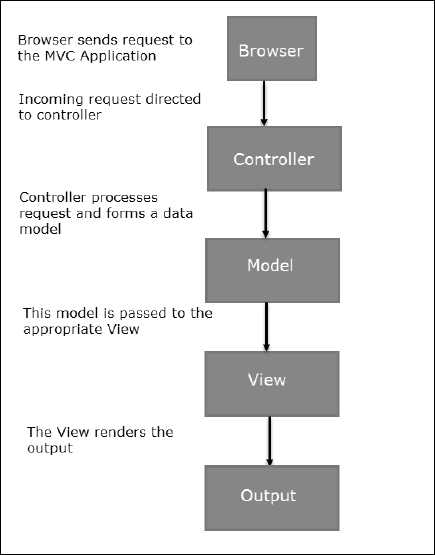
\includegraphics[width=0.5\textwidth]{images/ch2/mvc_flow.jpg}%
    \caption[MVC Flow Diagram]{MVC Flow Diagram}\cite{ha004}\label{fig: MVC Flow Diagram}%
  \end{figure}
\newpage
\textbf{Flow Steps}
\newline{\textbf{Step1}}
\newline{The client browser sends request to the MVC Application.}
\newline{\textbf{Step2}}
\newline{Global.ascx receives this request and performs routing based on the URL of the incoming request using the RouteTable, RouteData, UrlRoutingModule and MvcRouteHandler objects.}
\newline{\textbf{Step3}}
\newline{This routing operation calls the appropriate controller and executes it using the IControllerFactory object and MvcHandler object's Execute method.}
\newline{\textbf{Step4}}
\newline{The Controller processes the data using Model and invokes the appropriate method using ControllerActionInvoker object}
\newline{\textbf{Step5}}
\newline{The processed Model is then passed to the View, which in turn renders the final output.}
\subsection{PayPal}
\hspace{2cm} PayPal provides an easy and quick way to send and request money online. You can transfer money (abroad) to family, friends, online shops, and auction sites like eBay.
\newline{\textbf{Online payments}}
\newline{All you need to send money to family or friends is the email address of the recipient. By registering your credit card or bank account with your PayPal account you can send payments using the option.} \cite{ha005}
\newline{\textbf{Send and Request Money}}
\newline{The money will be credited to the recipient's account and can then be transferred to a bank account, or used to make a payment.
If you shop online and see the PayPal logo on the merchant's website, it means you can pay using PayPal. Just select PayPal at the checkout. You will be asked to log in to your account and confirm the payment. Your financial information will never be visible to sellers or online shops.}
\newline{\textbf{To receive money online}}
\newline{Anyone can send money to you using your email address. Your email address is linked to your personal PayPal account. You will receive an email notification whenever you receive a payment and the payment will be shown on your account.
Online shops that offer PayPal as a payment option can post the PayPal logo on their website. There are various ways to offer PayPal as a payment option, like Pay Now and Shopping Cart.
If you receive a payment through PayPal, PayPal 'll send you a notification by email. The money will be credited to your PayPal balance. You can transfer the money to your bank account or use it to make a payment yourself.} \newline
{\textbf{Fees}}
\newline{Opening a PayPal account is free. Fees will be charged depending on the payment you make:}
\begin{itemize}
  \item {\textbf{Personal payments}}
  \newline{Payments to friends and family are free provided you use your PayPal balance or bank account to send these payments. If you use your credit card, the recipient will be charged the associated fees. However, you as sender can state that you will pay these fees.}
  \item {\textbf{Commercial  payments}}
  \newline{If you buy an item, the recipient will be charged the associated fees. }
\end{itemize}
\textbf{Benefits of Using PayPal}
\begin{enumerate}
  \item {\textbf{Speed}} 
  \newline{PayPal transfers between sellers are instant, and transfers from PayPal accounts to bank accounts can take as little as 24 hours.}
  \item {\textbf{Affordability}}  
  \newline{The fee to use PayPal is 30 cents per transaction, plus 3 per cent of the total amount of the transaction.}
\end{enumerate}
\subsection{Stripe}
\hspace{2cm} Stripe builds the most powerful and flexible tools for internet commerce. Whether you’re creating a subscription service, an on-demand marketplace, an e-commerce store, or a crowdfunding platform, Stripe’s meticulously designed APIs and unmatched functionality help you create the best possible product for your users. Millions of the world’s most innovative technology companies are scaling faster and more efficiently by building their businesses on Stripe. Platforms use Stripe Connect to accept money and pay out to third parties. Connect provides a complete set of building blocks to support virtually any business model, including on-demand businesses, e-commerce, crowdfunding, and travel and events.  \cite{ha006} \newline \newline
\textbf{Features}
\begin{enumerate}
  \item {\textbf{Integrate quickly}} 
  \newline{Building the payments infrastructure for your platform used to be a big undertaking no longer. Take advantage of pre-made UI components to launch faster and simplify operations. Sign up new users on your platform and get them paid quickly.}
  \item {\textbf{Customize}}  
  \newline{Connect is API-first and lets you design the best experience for your platform. You can customize onboarding, set payout timing, allow complex money movement, and get integrated financial reporting. You own the experience from end to end.} \newline
\end{enumerate}
\textbf{Routing Payments} \newline
Connect will automatically track balances, batch earnings into payouts, time transfers with local cutoffs, and retry failed transfers. You can also incorporate advanced flows like Account Debits, one-to-many payments, and others. Connect’s payout engine lets you specify payout timing for your users, and includes Instant Payouts, which allows your users to receive funds within minutes. Connect lets you get recipients paid faster and removes errors and reconciliation work.

\subsection{Angular 9}
Angular is a way to build applications for any deployment target. For web, mobile web, native mobile and native desktop. \newline
It builds features quickly with simple, declarative templates. Extend the template language with your own components and use a wide array of existing components. Get immediate Angular-specific help and feedback with nearly every IDE and editor. All this comes together so you can focus on building amazing apps rather than trying to make the code work. \newline

 \begin{figure}[http]%
    \center%
    
\includegraphics[width=0.5\textwidth]{images/ch2/Angular.png}%
    \caption[Angular]{Angular}\label{fig: Angular}%
  \end{figure}

\textbf{Features} \cite{ha007}
\begin{itemize}
    \item {\textbf{Cross Platform}}
      \begin{itemize}
        \item {\textbf{Progressive Web Apps}}
        \newline{Use modern web platform capabilities to deliver app-like experiences. High performance, offline, and zero-step installation.}
        \item {\textbf{Native}}
        \newline{Build native mobile apps with strategies from Cordova, Ionic, or NativeScript.}
        \item {\textbf{Desktop}}
        \newline{Create desktop-installed apps across Mac, Windows, and Linux using the same Angular methods you've learned for the web plus the ability to access native OS APIs.}
    \end{itemize}
    \item {\textbf{Speed And Performance}}
      \begin{itemize}
        \item {\textbf{Code Generation}}
        \newline{Angular turns your templates into code that's highly optimized for today's JavaScript virtual machines, giving you all the benefits of handwritten code with the productivity of a framework.}
        \item {\textbf{Universal}}
        \newline{Serve the first view of your application on Node.js®, .NET, PHP, and other servers for near-instant rendering in just HTML and CSS. Also paves the way for sites that optimize for SEO.}
        \item {\textbf{Code Splitting}}
        \newline{Angular apps load quickly with the new Component Router, which delivers automatic code-splitting so users only load code required to render the view they request.}
    \end{itemize}
    \item {\textbf{Productivity}}
    \begin{itemize}
        \item {\textbf{Templates}}
        \newline{Quickly create UI views with simple and powerful template syntax.}
        \item {\textbf{Angular CLI}}
        \newline{Command line tools: start building fast, add components and tests, then instantly deploy.}
        \item {\textbf{IDEs}}
        \newline{Get intelligent code completion, instant errors, and other feedback in popular editors and IDEs.}
    \end{itemize}
    \item {\textbf{Full Development Story}}
    \begin{itemize}
        \item {\textbf{Animation}}
        \newline{Create high-performance, complex choreographies and animation timelines with very little code through Angular's intuitive API.}
        \item {\textbf{Accessibility}}
        \newline{Create accessible applications with ARIA-enabled components, developer guides, and built-in a11y test infrastructure.}
        \item {\textbf{Testing}}
        \newline{With Karma for unit tests, you can know if you've broken things every time you save. And Protractor makes your scenario tests run faster and in a stable manner.} 
    \end{itemize}
\end{itemize}

\textbf{Angular 9 Ivy} \newline
Angular 9’s compiling and rendering engine is known as Ivy. The older versions of Angular made use of View Engine. The bundle size produced by the View Engine is very large but with Ivy, this bundle has considerably reduced thereby helping Angular overcome its bundle issues. \newline

\textbf{Benefits} 
\begin{itemize}
    \item Smaller bundle size.
    \item Very helpful when it comes to debugging:
    \newline{With Angular 9, you will not have to debug through the framework, but rather, you can do it on the component itself which helps you debug your code instantly.}
    \begin{figure}[http]%
    \center%
    
\includegraphics[width=0.5\textwidth]{images/ch2/Debugging.jpg}%
    \caption[Debugging]{Debugging}\label{fig: Debugging}%
  \end{figure}
    \item Faster testing.
    \item Improved CSS class and style binding.
    \item Improved type checking.
    \item Improved build errors.
    \item Improved build times, enabling AOT on by default.
\end{itemize}